\documentclass[12pt]{article}
\usepackage[utf8]{inputenc}
\usepackage{parskip}
\usepackage{markdown}
\usepackage{hyperref}
\usepackage{listings}
\usepackage{color}
\usepackage[subtle]{savetrees}
\usepackage{verbatim}
\usepackage{blindtext}

\title{\vspace{-2cm} \textbf{Session 3 - Fun Logics} \\ UCAS Program 2020}

\author{Chloe Lau}
\date{August 2020}

\begin{document}
\setlength{\parindent}{4ex}
\setlength{\parskip}{1em}

\maketitle

\section{What is Logic?}
Logic isn't just a particular way of thinking, it is based on relating facts and introducing a result from the compilation of facts. Philosophical Logic, yet is very related to how we make sense of things, and Mathematical Logic, enhances our thinking to produce higher level proofs.

\section{Now, Think With Logic}
Now that you know what is Logic, we will be doing some Logical Puzzles, but in contrary to scribbles and just pure thinking that you usually do, you would need to lay out your thinking process, step by step, in written form.

You can lay out your steps on paper, your iPads, or on Google Docs.

Imagine this is an exam, so please keep your scribbles clear and make sure others would make sense of it.

You will be asked to talk about your thinking process at the end of the task, so \textbf{think} about it!

Ready? Let's delve into the wonders of Logic now!


\newpage
\subsection{CSAT 2019, Q2}
\begin{center}
    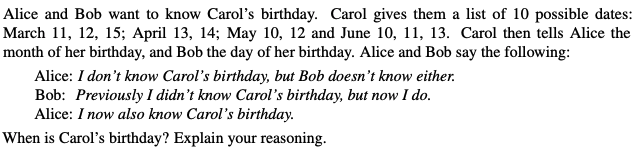
\includegraphics[scale=0.6]{csat19-2.png}
\end{center}

Space for some scribbling:

\newpage
\subsection{MAT 2007, Q6}
\begin{center}
    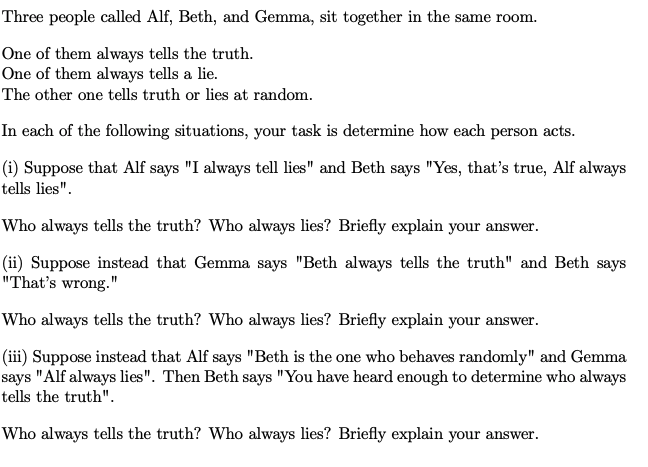
\includegraphics[scale=0.57]{mat07-6.png}
\end{center}

Space for some scribbling:

\end{document}
